\section{Цель работы}

Изучение связи между видом свободного процесса в электрической
цепи и расположением ее собственных частот (корней
характеристического уравнения) на комплексной плоскости;
экспериментально определить собственные частота и добротности
RLC-контура по осциллограммам.





\section{Приборы и материалы}

\begin{itemize}
    \item мультиметр;
    \item осциллограф;
    \item набор резисторов и реостат;
    \item 2 конденсатора;
    \item катушка;
    \item соединительные провода.
    \item Схема для исследования, изображенная на рис. \ref*{fig:scheme_1}.
\end{itemize}

\begin{figure}[!h]
    \centering
    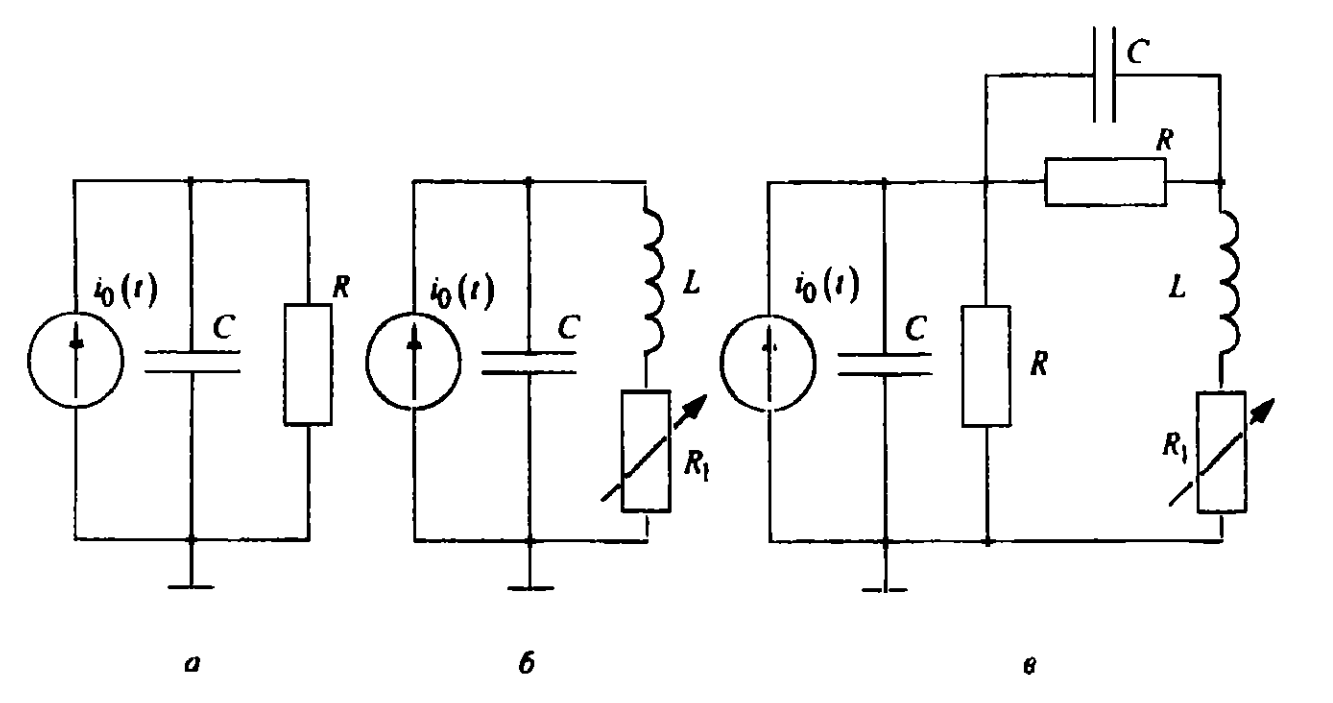
\includegraphics[width=\textwidth]{scheme_1.png}
    \caption{Схема для исследования}
    \label{fig:scheme_1}
\end{figure}

$C = 0,02$ мкФ, $L = 25$ мГн, $R = 5$ кОм, $R_1 = 0-4,7$ кОм.